\section{Drivetrain}
\label{sec:drivetrain}

The drivetrain has to carry a \qty{0.97}{kg} robot up the \ang{33.4} slope as fast as possible. The kit motors were too slow for that, so we bought inexpensive gearmotors. We chose them by first bounding the options with three physical limits: the traction the tracks can transmit (Section~\ref{sec:traction-bound}), the force needed to climb (Section~\ref{sec:holding-bound}) and the current the electronics can supply (Section~\ref{sec:current-bound}). We then picked the gear ratio with the shortest predicted climb among the motors left (Section~\ref{sec:gear-ratio}).

\subsection{Upper bound on torque: traction}
\label{sec:traction-bound}

The tracks can push along the ramp only until they slip, at the static friction force $F_f$ (Fig.~\ref{fig:fbd}). The total drive force $F$ is therefore capped by the maximum available traction:
\begin{equation}
  F \le \mu_s N
  \label{eq:traction}
\end{equation}
where the normal force is $N = m g \cos\ang{33.4}$ on the ramp and $N = m g$ on the mesa. Each motor drives one track through a sprocket of \qty{50}{mm} diameter ($r = \qty{25}{mm}$) and supplies half of $F$, so the torque per motor at which the tracks start to slip is $\mu_s N r / 2$ at the sprocket. We estimated $\mu_s = 1.2$ to be the most any tread material on the ramp could reasonably give, since that is about the highest static friction coefficient that surfaces engineered for grip, such as tires, reach. On the ramp the maximum available traction is then \qty{9.5}{N}, and no motor can usefully deliver more than \qty{0.12}{N.m} at the sprocket (Table~\ref{tab:traction}).

\begin{figure}[htbp]
  \centering
  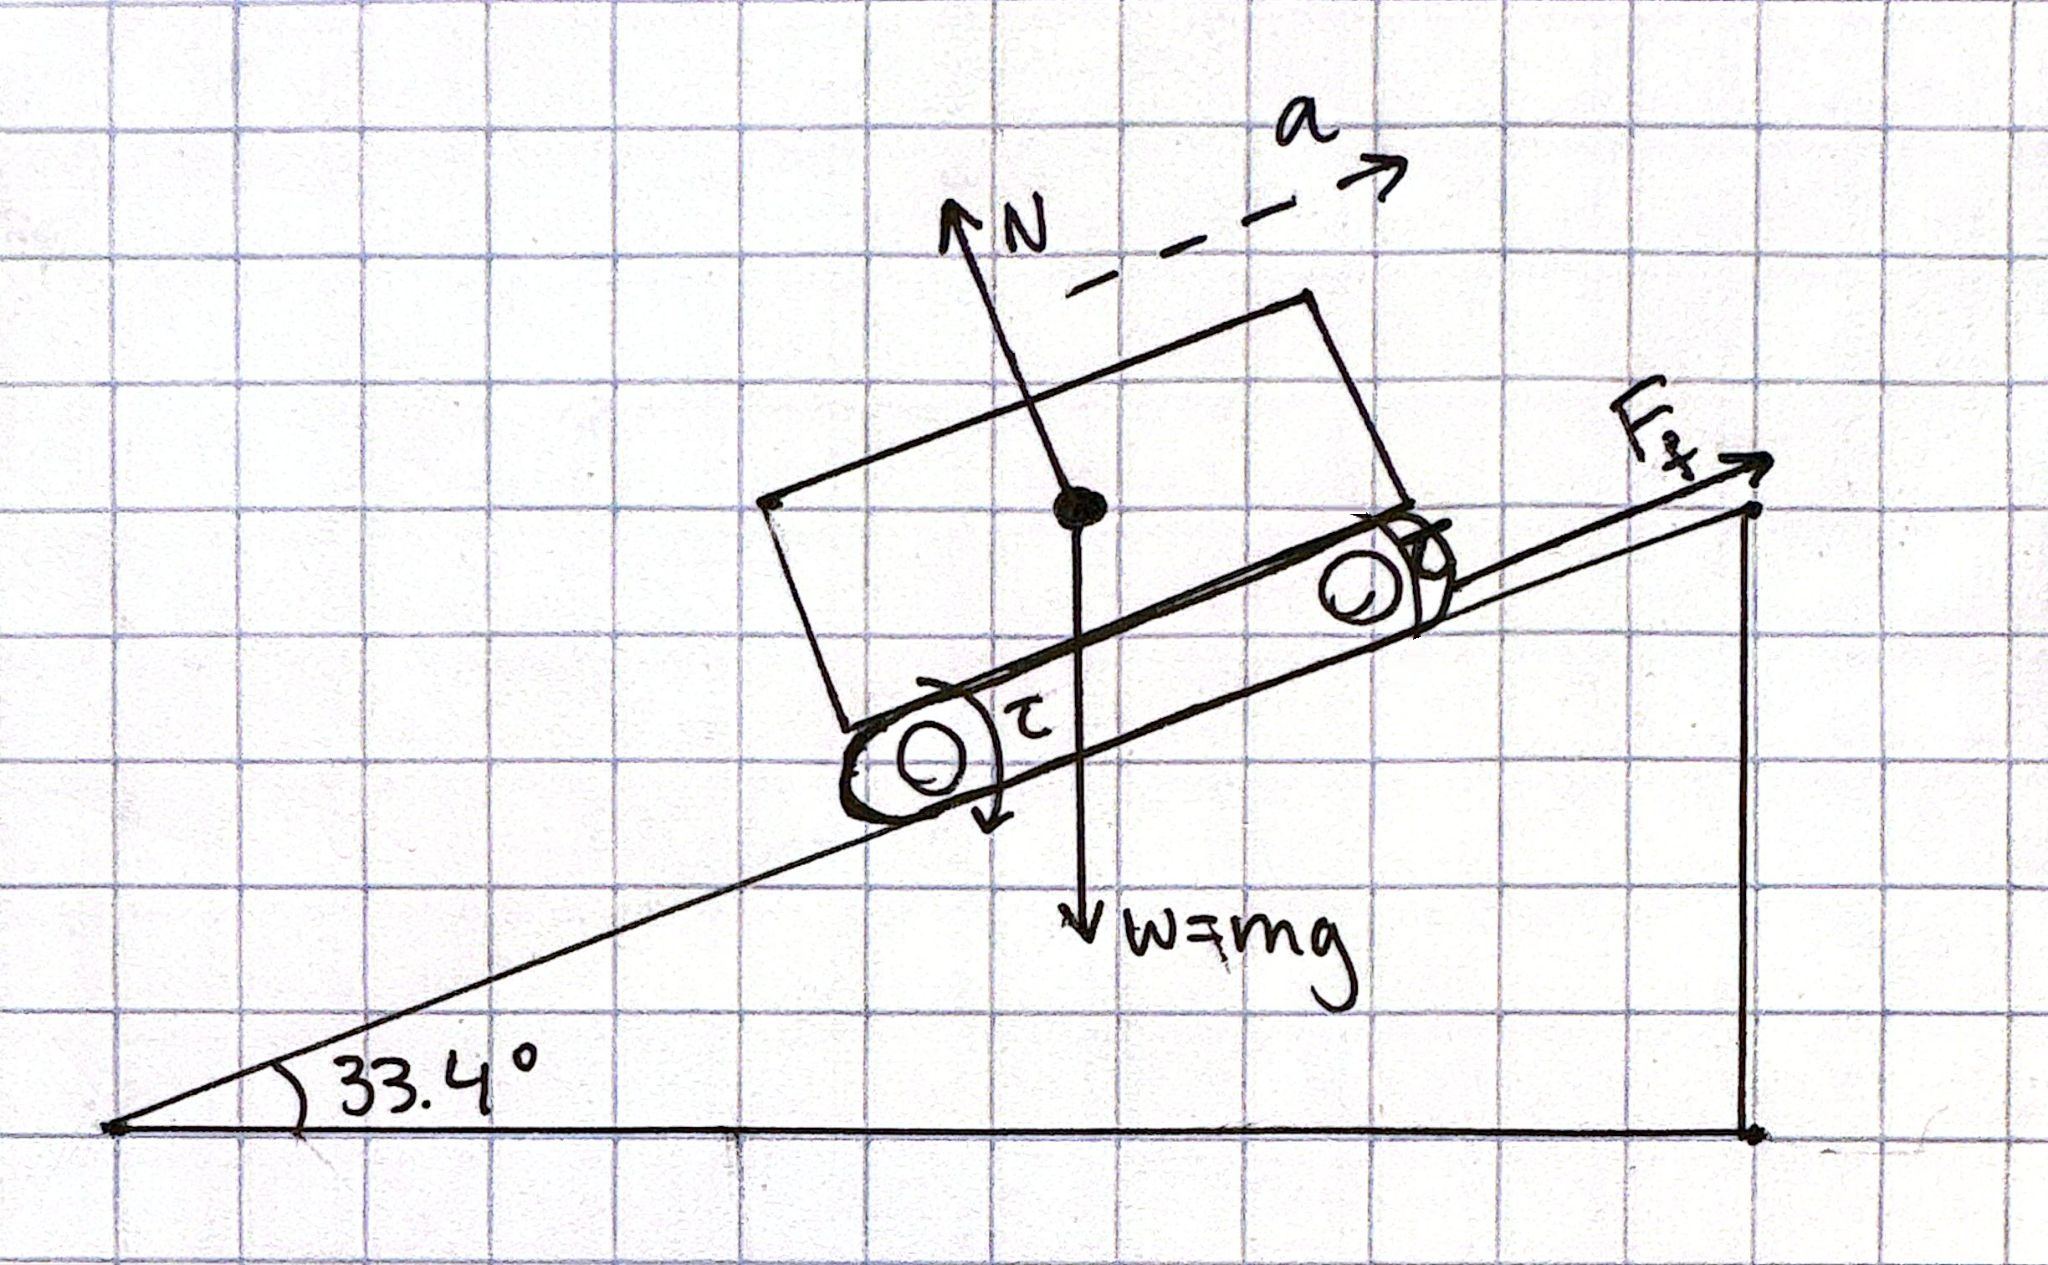
\includegraphics[width=0.58\textwidth]{fig03_fbd.jpg}
  \caption{Forces on the robot while it climbs. Friction at the tracks, $F_f$, is the only force pushing it up the ramp.}
  \label{fig:fbd}
\end{figure}

A real drivetrain also loses torque to resistance in the tracks, axles and couplers (Section~\ref{sec:holding-bound}), and we could not calculate how much before the drivetrain was built. The motors must supply that loss on top of the force the tracks transmit, so we allowed stall force up to three times the maximum available traction. The factor of 3 is a judgment call, generous on purpose because the losses were unknown. Physically, it means a motor at this bound could lose two thirds of its stall force inside the drivetrain and still deliver the full maximum available traction at stall. Excess stall force is not wasted outright: a motor's force falls as it speeds up (Eq.~\eqref{eq:motor}), so it only makes the tracks slip for the first part of the climb.

\begin{table}[htbp]
  \centering
  \caption{The most force the tracks of a \qty{0.97}{kg} robot can transmit before slipping (maximum available traction), and the matching maximum usable torque per motor at a \qty{50}{mm} sprocket, for three assumed values of the maximum $\mu_s$.}
  \label{tab:traction}
  \begin{tabular}{@{}c cc cc@{}}
    \toprule
    & \multicolumn{2}{c}{Ramp} & \multicolumn{2}{c}{Mesa} \\
    \cmidrule(lr){2-3}\cmidrule(l){4-5}
    Assumed & Max.\ static & Max.\ usable torque & Max.\ static & Max.\ usable torque \\
    maximum $\mu_s$ & friction force (\unit{N}) & per motor (\unit{N.m}) & friction force (\unit{N}) & per motor (\unit{N.m}) \\
    \midrule
    0.8 & 6.36 & 0.079 & 7.61  & 0.095 \\
    1.0 & 7.94 & 0.099 & 9.52  & 0.119 \\
    1.2 & 9.53 & 0.119 & 11.42 & 0.143 \\
    \bottomrule
  \end{tabular}
\end{table}

\subsection{Lower bound on torque: holding on the slope}
\label{sec:holding-bound}

Gravity pulls the robot down the ramp with $m g \sin\ang{33.4} = \qty{5.24}{N}$. To start from rest and climb, the motors' stall force must exceed that pull plus every other resistance:
\begin{equation}
  F_\mathrm{stall} > k_r\, m g \sin\ang{33.4}
  \label{eq:holding}
\end{equation}
Here $k_r$ is the total resistance to climbing as a multiple of gravity's pull, so $k_r - 1$, which we call the extra resistance, counts every resistance besides gravity and the gearbox losses, which Section~\ref{sec:gear-ratio} counts separately as the gearbox efficiency $\eta_\mathrm{g}$. A value of $k_r = 1$ would be a robot with no extra resistance; $k_r = 1.25$ means the extra resistance adds a quarter of gravity's pull, \qty{1.31}{N}. We could not calculate $k_r$ from first principles, because it comes from friction and deflection throughout the drivetrain and from rubbing on the side wall (Section~\ref{sec:drivetrain-result}). A motor that only just clears Eq.~\eqref{eq:holding} climbs, but with so little force to spare for acceleration it never reaches its full speed on a \qty{1.524}{m} ramp.

\subsection{Upper bound on motor size: current}
\label{sec:current-bound}

A bigger motor makes more power only by drawing more current. A brushed DC motor with winding resistance $R_\mathrm{w}$ stalls at $I_\mathrm{stall} = V / R_\mathrm{w}$ and delivers its peak mechanical power at half its stall torque and half its no-load speed:
\begin{equation}
  P_\mathrm{max} = \frac{V I_\mathrm{stall}}{4}
  \label{eq:pmax}
\end{equation}
The voltage is fixed by the kit's 2S pack, so stall current is a proxy for motor size: the largest viable motors are those whose current the electronics can supply. The motors will stall briefly at the start of every climb and could stall for a long time in a pushing match. Two components limit $I_\mathrm{stall}$ (Table~\ref{tab:current}).

\paragraph{Driver}
The TB6612FNG driver we had on hand is rated for \qty{1.2}{A} continuous and \qty{3.2}{A} peak per channel~\cite{tb6612}. A continuous stall, though unlikely, could occur in a pushing match, which caps $I_\mathrm{stall}$ at \qty{1.2}{A} per motor. Because most stalls are brief, up to \qty{3.2}{A} is acceptable.

\paragraph{Pack}
The 7805 linear regulator steps an input between 7 and \qty{25}{V} down to the \qty{5}{V} the Photon runs on~\cite{reg7805}. Below \qty{7}{V} input, the \qty{5}{V} supply cannot be held and the Photon behaves erratically or cuts out, which loses the match. The voltage sag from the motors in a likely worst case therefore must not pull the pack below \qty{7}{V}. The terminal voltage of a battery with open-circuit voltage $\mathcal{E}$ and internal resistance $R_\mathrm{int}$ is
\begin{equation}
  V_\mathrm{term} = \mathcal{E} - I_\mathrm{pack} R_\mathrm{int}
  \label{eq:vterm}
\end{equation}
so with both motors at stall the pack sags by $\Delta V_\mathrm{sag} = 2 I_\mathrm{stall} R_\mathrm{int}$, and the largest stall current per motor that keeps the pack above \qty{7}{V} is
\begin{equation}
  I_\mathrm{stall,max} = \frac{\mathcal{E} - \qty{7}{V}}{2 R_\mathrm{int}}
  \label{eq:istall-max}
\end{equation}
Taking $R_\mathrm{int} \approx \qty{0.15}{\ohm}$ \tbd{replace with our measured value from the voltage-drop test} and $\mathcal{E} = \qty{7.4}{V}$, Eq.~\eqref{eq:istall-max} gives $I_\mathrm{stall,max} = \qty{1.3}{A}$. The value \qty{7.4}{V} is the nominal 2S voltage; a 2S pack runs from \qty{8.4}{V} full to a usual cutoff of \qty{6.0}{V}~\cite{cell}. But even with both motors stalled throughout, six \qty{30}{s} runs draw only about \qty{0.14}{A.h}, a few percent of the pack's capacity, so the pack stays near nominal. The best case, a full pack at $\mathcal{E} = \qty{8.4}{V}$, allows \qty{4.7}{A} per motor.

\begin{table}[htbp]
  \centering
  \caption{Limits on the stall current of each motor, $I_\mathrm{stall}$, from the driver and from the pack.}
  \label{tab:current}
  \begin{tabularx}{\textwidth}{@{}L L c L c@{}}
    \toprule
    & \multicolumn{2}{c}{Worst case} & \multicolumn{2}{c}{Best case} \\
    \cmidrule(lr){2-3}\cmidrule(l){4-5}
    Limiting component & Condition & Max.\ $I_\mathrm{stall}$ (\unit{A}) & Condition & Max.\ $I_\mathrm{stall}$ (\unit{A}) \\
    \midrule
    Driver (TB6612FNG) & Stall held, as in a pushing match & 1.2 & Brief stall at the start of a climb & 3.2 \\
    Pack (7805 drops out below \qty{7.0}{V}) & Pack at \qty{7.4}{V} & 1.3 & Full pack at \qty{8.4}{V} & 4.7 \\
    \bottomrule
  \end{tabularx}
\end{table}

We wanted a motor wound for close to our pack voltage. The match does not have to be exact: above its rated voltage a motor's speed and stall current rise in proportion, so a \qty{6}{V} motor on our \qty{7.4}{V} pack runs about \qty{23}{\percent} faster and draws about \qty{23}{\percent} more current, which Table~\ref{tab:current} must allow. A \qty{37}{mm} gearmotor stalls at \qty{5.5}{A} even at its \qty{12}{V} rating~\cite{pololu37d}, several times our worst-case limit. Pololu's \qty{25}{mm}, \qty{6}{V} gearmotors stall at about \qty{2.0}{A}~\cite{pololu25d}. The cheaper \qty{25}{mm} motors we found on Amazon are rated at \qty{2.7}{W}~\cite{meccanixity}; taking that as the peak power on our pack, Eq.~\eqref{eq:pmax} gives $I_\mathrm{stall} = 4 P_\mathrm{max} / V = \qty{1.46}{A}$, about \qty{1.5}{A}. That is just above the worst-case limit and well inside the best case, so of the sizes we compared, a \qty{25}{mm} gearmotor wound for \qty{6}{V} fits the kit pack best.

\subsection{Choosing the gear ratio inside the bounds}
\label{sec:gear-ratio}

The listing offers \qty{25}{mm} \qty{6}{V} gearmotors with ratios from 1:4.4 to 1:500~\cite{meccanixity}. Changing the ratio on the same base motor only reallocates power between speed and torque. Too low a ratio gives too little torque to accelerate the robot against gravity and drivetrain resistance. Too high a ratio wastes gearing on torque the tracks cannot use and limits top speed. To find the optimum, we wrote the estimated climb time as a function of gear ratio, $t_\mathrm{climb}(G)$, and evaluated it for every version on sale.

\paragraph{Motor model}
A brushed DC motor makes torque in proportion to its current, and the pack voltage divides between the winding resistance and the back-EMF the spinning motor generates. In SI units the torque constant and the back-EMF constant are the same number, $k_\mathrm{t}$, so $\tau_\mathrm{m} = k_\mathrm{t} I_\mathrm{m}$ and $V = I_\mathrm{m} R_\mathrm{w} + k_\mathrm{t}\, \omega_\mathrm{m}$. Eliminating $I_\mathrm{m}$ shows torque falling linearly from its stall value to zero at the no-load speed. We had to choose before we had a motor to test, so we took the no-load speed from the listing, about \qty{6000}{\rpm} (\qty{625}{rad/s}) at \qty{6}{V}, and our estimated stall current of \qty{1.5}{A} on the \qty{7.4}{V} pack:
\begin{equation}
  k_\mathrm{t} = \frac{\qty{6}{V}}{\qty{625}{rad/s}} = \qty{0.0096}{N.m/A}, \qquad
  R_\mathrm{w} = \frac{\qty{7.4}{V}}{\qty{1.5}{A}} = \qty{4.9}{\ohm}
  \label{eq:k}
\end{equation}
The gearbox divides speed by $G$ and multiplies torque by $G$, losing a fraction of the torque to the gearbox efficiency $\eta_\mathrm{g}$, and the sprocket of radius $r$ turns shaft torque into track force. For both motors together, the drive force at robot speed $v$ is
\begin{equation}
  F(v) = F_\mathrm{stall}\left(1 - \frac{v}{v_0}\right), \qquad
  F_\mathrm{stall} = \frac{2 \eta_\mathrm{g} k_\mathrm{t} G V}{R_\mathrm{w} r}, \qquad
  v_0 = \frac{V r}{k_\mathrm{t} G}
  \label{eq:motor}
\end{equation}
Raising $G$ raises $F_\mathrm{stall}$ and lowers $v_0$ in the same proportion.

\paragraph{Equation of motion}
Two kinds of resistance oppose the drive force. Internal losses eat motor torque before it reaches the ramp: friction within the treads, the side guards rubbing on the treads, and the energy spent flexing the couplers as they turn. External resistance acts on the robot directly, as gravity does: friction and small collisions against the side wall. We lump both into $k_r$ (Eq.~\eqref{eq:holding}), so the total resistance is $F_\mathrm{r} = k_r\, m g \sin\ang{33.4}$. The drive force also cannot exceed the maximum available traction, $\mu_s m g \cos\ang{33.4}$ (Eq.~\eqref{eq:traction}); for $t_\mathrm{climb}(G)$ we took $\mu_s = 1.0$, the middle row of Table~\ref{tab:traction}. Newton's second law along the ramp is then
\begin{equation}
  m \frac{dv}{dt} = \min\!\left[F(v),\ \mu_s m g \cos\ang{33.4}\right] - F_\mathrm{r}
  \label{eq:climb}
\end{equation}
Gear losses grow with the load, so $\eta_\mathrm{g}$ scales the motor force, while $k_r$ is a constant drag. Subtracting internal losses after capping the drive force overstates them while the tracks slip, so the model errs slow, and it assumes full motor duty from the start.

\paragraph{Solving for the climb time}
$t_\mathrm{climb}(G)$ is the time Eq.~\eqref{eq:climb}, started from rest, takes to carry the robot \qty{1.524}{m}. The minimum splits the climb into two phases. At low speed the tracks slip and the robot accelerates uniformly at the traction limit; for the \qty{280}{\rpm} version this lasts \qty{0.17}{s} and covers \qty{4}{cm}. After that the motors limit the force, Eq.~\eqref{eq:climb} becomes linear, and the speed approaches exponentially the speed $v_t = v_0(1 - F_\mathrm{r}/F_\mathrm{stall})$ at which drive force balances resistance, with time constant $t_0 = m v_0 / F_\mathrm{stall} = \qty{0.05}{s}$. We integrated once more for position and found the time to cover \qty{1.524}{m} by bisection.

\paragraph{Why there is an optimum}
The robot spends nearly the whole climb close to $v_t$ (\qty{0.63}{m/s} for the \qty{280}{\rpm} version with $\eta_\mathrm{g} = 0.7$ and $k_r = 1$), so the fastest climb comes from the largest $v_t$. Substituting the stall force and no-load speed into $v_t$ and setting its derivative with respect to $G$ to zero, $v_t$ is largest when
\begin{equation}
  F_\mathrm{stall} = 2 F_\mathrm{r}
  \label{eq:optimum}
\end{equation}
At that gear ratio the motors climb at half their no-load speed, where a DC motor delivers its peak power. More reduction makes the motors strong but slow. Less reduction leaves so little force to spare over $F_\mathrm{r}$ that the motors must run close to stall to keep climbing. For the three combinations of $\eta_\mathrm{g}$ and $k_r$ in Fig.~\ref{fig:gear}b, Eq.~\eqref{eq:optimum} puts the optimum between the \qty{620}{\rpm} (1:9.6) and \qty{280}{\rpm} (1:21.3) versions.

\paragraph{Applying the bounds}
Every version shares the same base motor, so all of them meet Section~\ref{sec:current-bound}. The torque bounds of Sections~\ref{sec:traction-bound} and~\ref{sec:holding-bound} leave three candidates: the 170, 280 and \qty{620}{\rpm} versions (Fig.~\ref{fig:gear}a). The \qty{280}{\rpm} version (1:21.3) gives the shortest estimated climb (Fig.~\ref{fig:gear}b). It stays fastest for every combination of $\eta_\mathrm{g}$ from 0.5 to 0.8 and $k_r$ from 1.0 to 1.25 except the most optimistic corner, $\eta_\mathrm{g}$ of 0.75 or more with $k_r$ of about 1.1 or less, where the \qty{620}{\rpm} version is slightly faster. Nothing is sold between 280 and \qty{620}{\rpm}.

\begin{figure}[htbp]
  \centering
  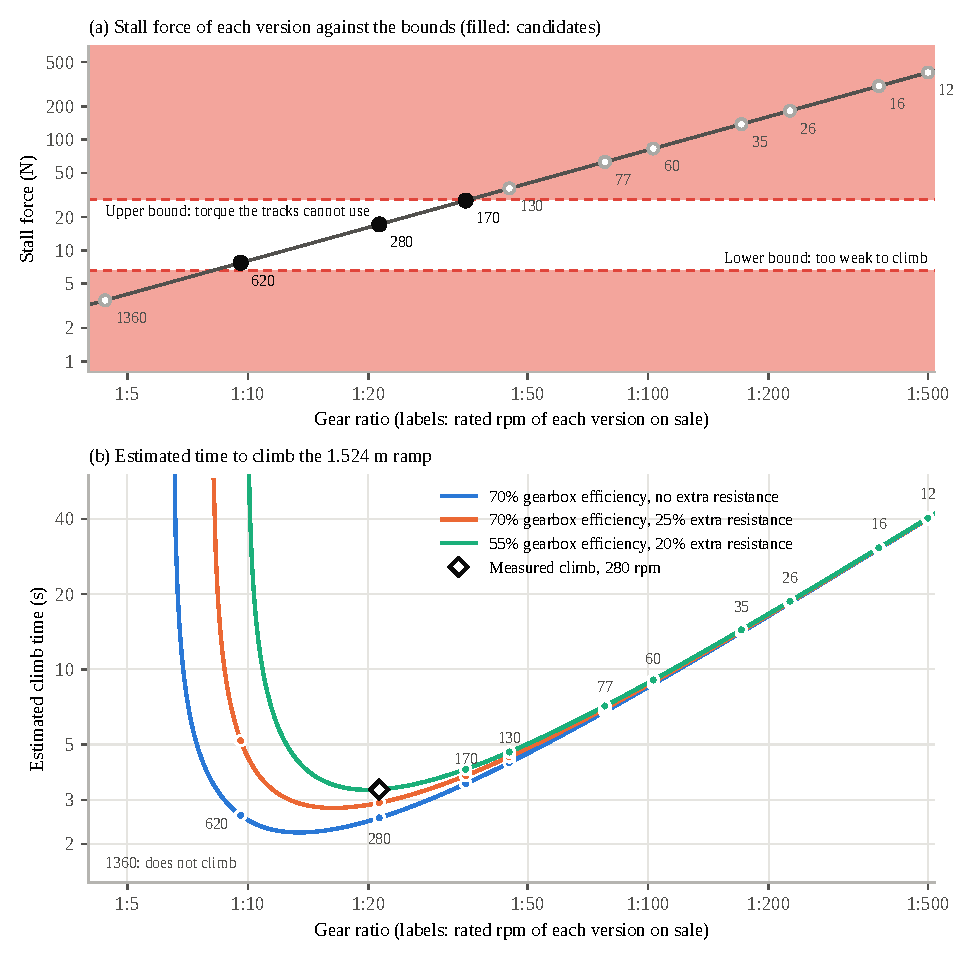
\includegraphics[width=0.74\textwidth]{fig04_gear_ratio.pdf}
  \caption{Choosing the gear ratio. (a) Stall force of each version on the \qty{7.4}{V} pack ($\eta_\mathrm{g} = 0.7$). Only the 170, 280 and \qty{620}{\rpm} versions fall between the lower bound (Section~\ref{sec:holding-bound}) and the upper bound (Section~\ref{sec:traction-bound}). (b) Estimated climb time $t_\mathrm{climb}(G)$ from Eq.~\eqref{eq:climb}. The \qty{280}{\rpm} version is fastest in all three cases, and our measured \qty{3.3}{s} climb falls on the curve for \qty{55}{\percent} gearbox efficiency with \qty{20}{\percent} extra resistance.}
  \label{fig:gear}
\end{figure}

\subsection{Result}
\label{sec:drivetrain-result}

We bought and ran the \qty{280}{\rpm} version. We measured its stall current on a charged pack at \qty{1.4}{A}, close to the \qty{1.5}{A} we had estimated. In three stopwatch trials the robot climbed the ramp in about \qty{3.3}{s}. For the \qty{280}{\rpm} version, $t_\mathrm{climb}(G)$ gives 2.4 to \qty{3.8}{s} over our range of losses, $\eta_\mathrm{g}$ from 0.5 to 0.8 and $k_r$ from 1.0 to 1.25, and \qty{2.5}{s} with no extra resistance ($\eta_\mathrm{g} = 0.7$, $k_r = 1$). The measured time falls inside that range, so the model is consistent with the measurement. One climb time cannot separate the two losses: $\eta_\mathrm{g} = 0.55$ with $k_r = 1.2$, for example, gives \qty{3.3}{s}.

Several problems in our build add to that resistance. The side guards flexed into the treads and rubbed on them in every run (Section~\ref{sec:layout}). The tracks are tensioned tightly so they do not dip and scrape at the mesa edge (Section~\ref{sec:couplers}), which loads the sprockets and axles. The printed couplers flex as they turn, the treads have friction within themselves, and the robot rubs and knocks against the side wall it uses as a guide rail.
